%!TEX program = xelatex

% Presentazione finale delle tavole applicative per il corso di controllo dei robot
% Enrico Puglisi & Andrea Ryals

%!TEX root = ../main.tex
%
% PREAMBLE
\documentclass[10pt, english]{beamer}
\usetheme{metropolis}
\usepackage[english]{babel}
\usepackage[utf8]{inputenc}

% \usepackage{booktabs}
% \usepackage[scale=2]{ccicons}
% \usepackage{minted}
% \usepgfplotslibrary{dateplot}
% \usemintedstyle{trac}

%Utilities
\usepackage{multicol}
\usepackage{xcolor}
\usepackage{cancel}

% Graphics
\usepackage[absolute,overlay]{textpos}
\usepackage[font=scriptsize,labelfont=bf]{caption}
\usepackage{tabu}

%Videos
\usepackage{multimedia}

% Bibliography
\usepackage{multimedia}
\usepackage{csquotes}
\usepackage[backend=biber,style=numeric-comp,sorting=none]{biblatex}
\addbibresource{bib/biblio.bib}

%characters
\usepackage{gensymb}

%Math
\usepackage{breqn}
\setcounter{MaxMatrixCols}{20}

\newcommand\hcancel[2][black]{\setbox0=\hbox{$#2$}%
\rlap{\raisebox{.45\ht0}{\textcolor{#1}{\rule{\wd0}{1pt}}}}#2}

%% Title frame information
\title{Tavole applicative}
\subtitle{Corso di Controllo dei Robot}
\author[Puglisi, Ryals] % (optional, for multiple authors)
{E.~Puglisi \and A.~Ryals}
\institute[Università di Pisa] % (optional)
{Ingegneria robotica e dell'automazione\\
 Università di Pisa}
\date{\today}
\subject{Corso di Controllo dei robot}



\begin{document}
%
% Title page
\frame{\titlepage}
%
%Table of contents
\begin{frame}
\frametitle{Table of contents}
\begin{multicols}{2}
\tableofcontents
\end{multicols}
\end{frame}


%
%!TEX root = ../main.tex
%
\section[Delta robot]{Delta robot}
\begin{frame}

\end{frame}

\subsection{Direct kinematic}
\begin{frame}
\frametitle{Delta robot - Direct kinematic}
	\begin{figure}
		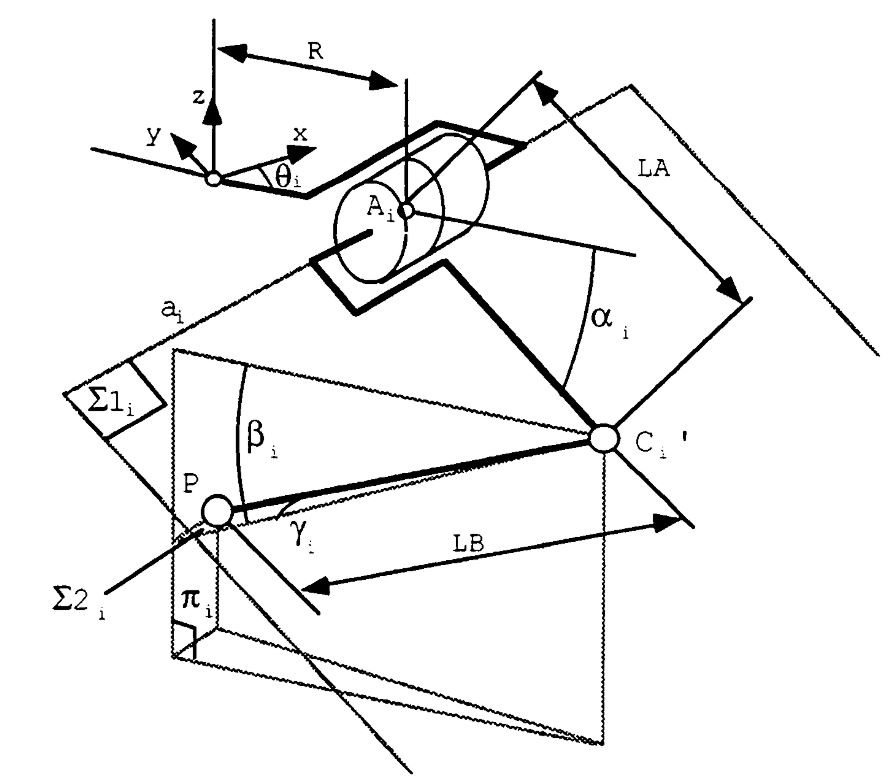
\includegraphics[width=.5\linewidth]{img/DeltaRobotClavelpg26.JPG}
	\end{figure}
\end{frame}
%
\begin{frame}
\frametitle{Delta robot - Direct kinematic}
	$C_i$ coordinates are given by the intersection of three circles of radius $L_A$ belonging to the plane $\pi_i$ and the sphere centered in $P$ having radius $L_B$.
	\[
	C_i =%
	\begin{pmatrix}
		(R + L_Acos\alpha_i)cos\theta_i\\
		(R + L_Acos\alpha_i)sin\theta_i\\
		-L_Asin\alpha_i
	\end{pmatrix}
	\]
	%
	Equation of the sphere centered in P:
	\begin{equation}
		(x - p_x)^2 + (y - p_y)^2 + (z - p_z)^2 = L_B
	\end{equation}
	%
	\begin{equation}
		((R + L_Acos\alpha_i)cos\theta_i - x^2) + ((R + L_Acos\alpha_i)sin\theta_i - y)^2 + (L_Asin\alpha_i + z)^2 = L_B^2
	\end{equation}

\end{frame}
\begin{frame}
	\frametitle{Delta robot - Direct kinematic}
	\begin{align}
		D_i &= R^2+2\,\cos\,q_{i}\,R\,l_{A}+{l_{A}}^2-{l_{B}}^2\\
		E_i &= \cos\theta _{i}\,\left(2\,R+2\,l_{A}\,\cos\,q_{i}\right)\\
		F_i &= \sin\theta _{i}\,\left(2\,R+2\,l_{A}\,\cos\,q_{i}\right)\\
		G_i &= -2\,l_{A}\,\sin\left(q_{i}\right)
	\end{align}
%
	\begin{align}
		H_1 &= E_{1}\,G_{2}-E_{2}\,G_{1}-E_{1}\,G_{3}+E_{3}\,G_{1}+E_{2}\,G_{3}-E_{3}\,G_{2}\\
		H_2 &= E_{2}\,F_{1}-E_{1}\,F_{2}+E_{1}\,F_{3}-E_{3}\,F_{1}-E_{2}\,F_{3}+E_{3}\,G_{2}\\
		H_3 &= D_{1}\,E_{2}-D_{1}\,E_{1}-D_{1}\,E_{3}+D_{3}\,E_{1}+D_{2}\,E_{3}-D_{3}\,E_{2}\\
		H_4 &= D_{2}\,F_{1}-D_{1}\,F_{2}+D_{1}\,F_{3}-D_{3}\,F_{1}-D_{2}\,F_{3}+D_{3}\,F_{2}\\
		H_5 &= F_{2}\,G_{1}-F_{1}\,G_{2}+F_{1}\,G_{3}-F_{3}\,G_{1}-F_{2}\,G_{3}+F_{3}\,G_{2}
	\end{align}
\end{frame}
%
\begin{frame}
\frametitle{Delta robot - Direct kinematic}
	\begin{align}
		L &= \frac{{H_{1}}^2+{H_{5}}^2}{{H_{2}}^2}+1\\
		M &= G_{1}-\frac{E_{1}\,H_{5}+F_{1}\,H_{1}}{H_{2}}+\frac{2\,H_{1}\,H_{3}+2\,H_{4}\,H_{5}}{{H_{2}}^2}\\
		N &= D_{1}-\frac{E_{1}\,H_{4}+F_{1}\,H_{3}}{H_{2}}+\frac{2\,{H_{3}}^2+2\,{H_{4}}^2}{{H_{2}}^2}
	\end{align}
\end{frame}
%
\begin{frame}
\frametitle{Delta robot - Direct kinematic}
End effector coordinates computation:
	\begin{equation}
		z_{1,2} = -\frac{M \pm \sqrt{M^2-4\,L\,N}}{2\,L}
	\end{equation}
	%
	Among the two solutions we pick the one with lower height that belongs to the Delta robot workspace.
	%
	\begin{align}
		x &= \frac{H_{4}}{H_{2}}-\frac{H_{5}\,\left(M-\sqrt{M^2-4\,L\,N}\right)}{2\,H_{2}\,L}\\
		y &= \frac{H_{3}}{H_{2}}-\frac{H_{1}\,\left(M-\sqrt{M^2-4\,L\,N}\right)}{2\,H_{2}\,L}
	\end{align}
\end{frame}
%
\subsection{Inverse kinematic}
\begin{frame}
	\frametitle{Delta robot - Inverse kinematic}
	\begin{align}
		A &= {L_{A}}^2-{L_{B}}^2-R^2+{x_{i}}^2+{y_{i}}^2+{z_{i}}^2\\
		B &= 2x_{i}-2R
	\end{align}
	%
	\begin{equation}
		z = \frac{A - Bx}{2\,z_{i}}
	\end{equation}
	%
	where:
	\begin{equation}
		x = \frac{b+\sqrt{b^2-a\,c}}{a}
	\end{equation}
	with:
	\begin{align}
		a &= {\left(2\,R-2\,x_{i}\right)}^2+4\,{z_{i}}^2\\
		b &= 4\,R\,{z_{i}}^2 + A\,B\\
		c &= A^2 - 4\,{L_{A}}^2\,{z_{i}}^2+4\,R^2\,{z_{i}}^2
	\end{align}
	%
	\begin{equation}
		q_i = -\mathrm{asin}\left(\frac{z}{L_{A}}\right)
	\end{equation}
\end{frame}
%
\subsection{Jacobian}
\begin{frame}
	\frametitle{Delta robot - Jacobian computation}
	\begin{equation}
		\left(\begin{array}{c} p-R_{b}\,\left(\overline{R}-L_{A}\,\cos\left(\overline{q_{i}}\right)\right)\\ p\\ p+L_{A}\,R_{b}\,\sin\left(\overline{q_{i}}\right) \end{array}\right)
	\end{equation}
\end{frame}
%
%!TEX root = ../main.tex
%
\section{Ball and plate}
\begin{frame}
	\frametitle{Ball and plate}
\end{frame}
%
\begin{frame}
\frametitle{Ball and plate}
%
\begin{figure}
		{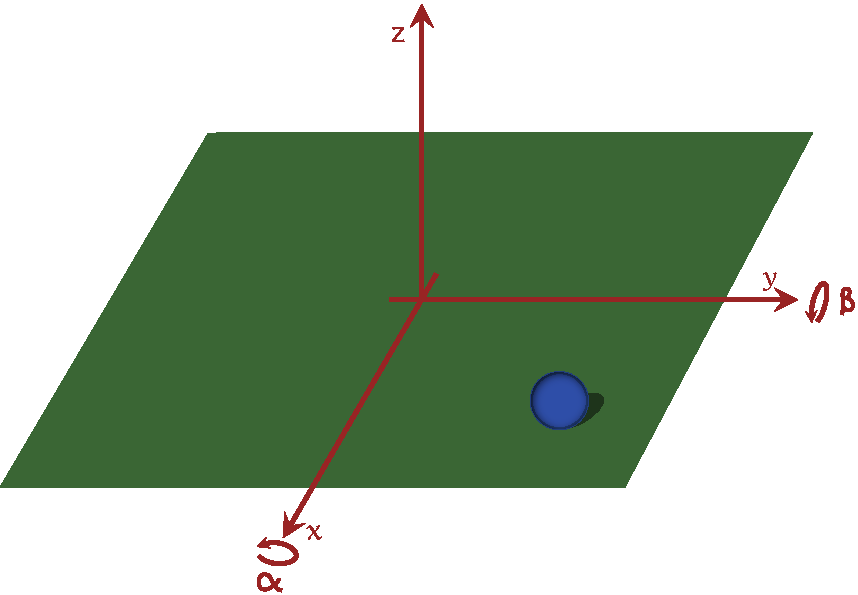
\includegraphics[width=.8\linewidth]{img/ballplate.pdf}}
		\caption{Coordinate frame of the ball and plate system}
		\label{fig:BallPlate}
\end{figure}
\end{frame}
%
\begin{frame}
\frametitle{Ball and plate - Parameters}
\begin{table}
\begin{center}
\begin{tabu} to \textwidth { | X[c] | X[c] | X[c] | }
	\hline
	\textbf{Parameter} & \textbf{Description} & \textbf{Value} \\
	\hline
	$m$ & Mass of the ball & $0.0109 \, Kg$ \\
	$r$ & Radius of the ball & $0.01 \, m$ \\
	$I_b$ & Ball inertia & $4.3563e^{-7} \, Kg\times m^2$ \\
	$l_p$ & Plate side & $0.6 \, m$ \\
	$I_p$ & Plate inertia & $0.175 \, Kg\times m^2$ \\
	\hline
\end{tabu}
\caption{Ball and plate geometric and dynamic parameters}
\label{tab:BallPlate_param}
\end{center}
\end{table}
\end{frame}
%
\subsection{Dynamic}
\begin{frame}
\frametitle{Ball and plate - Dynamic model}
%
The general form of Euler-Lagrange for dynamic equations is used to describe the system:
%
\begin{equation}
	\frac{d}{dt}\frac{\delta T}{\delta q_i} - \frac{\delta T}{\delta q_i} + \frac{\delta V}{\delta q_i} = Q_i
\end{equation}
%
Where $T$ is the kinetic energy, $V$ is the potential energy, $Q_i$ is the i-th generalized force and $q_i$ id the i-th generalized coordinate. As generalized force we consider two torques acting on the plate $(Q_\alpha = \tau_\alpha, Q_\beta = \tau_\beta)$. As generalized coordinates we select two ball position coordinates $[x, y]$ on the frame fixed to the plate and two plate inclination $[\alpha, \beta]$.
\end{frame}
%
\begin{frame}
\frametitle{Ball and plate - Dynamic model}
%
Kinetic energy of the ball:
\begin{equation}
	T_{b} = \frac{1}{2}mv^2 + \frac{1}{2}I_b\omega^2 = \frac{1}{2}\left(m+\frac{I_b}{r^2}\right)\left(\dot{x}^2+\dot{y}^2\right)
\end{equation}
%
Kinetic energy of the plate:
\begin{equation}
	T_{p} = \frac{1}{2}\left(I_b + I_p\right)\left(\dot{\alpha} + \dot{\beta}\right) + \frac{1}{2}m\left(\dot{\alpha}x + \dot{\beta}y\right)^2
\end{equation}
%
Potential energy:
\begin{equation}
	V = mgh = mg(x\,sin\alpha + y\,sin\beta)
\end{equation}
\end{frame}
%
\begin{frame}
\frametitle{Ball and plate - Dynamic model}
%
After some derivations we find the following non-linear system:
%
\begin{align}
	\left(m + \frac{I_b}{r^2}\right)\ddot{x} &- m\left(\dot{\alpha}\dot{\beta}y + \dot{\alpha}^2x\right)+mg\,sin\alpha = 0 \nonumber \\
	\left(m + \frac{I_b}{r^2}\right)\ddot{y} &- m\left(\dot{\alpha}\dot{\beta}x + \dot{\beta}^2y\right)+mg\,sin\beta = 0 \\
	\left(I_p + I_b + mx^2\right)\ddot{\alpha} &+ m\left(\ddot{\beta}xy + \dot{\beta}\left(\dot{x}y + x\dot{y}\right) + 2\dot{\alpha}\dot{x}x\right) +mgx\,cos{\alpha} = \tau_\alpha \nonumber \\
	\left(I_p + I_b + my^2\right)\ddot{\beta} &+ m\left(\ddot{\alpha}xy + \dot{\alpha}\left(\dot{x}y + x\dot{y}\right) + 2\dot{\beta}\dot{y}y\right) +mgy\,cos{\beta} = \tau_\beta \nonumber
\end{align}
%
\end{frame}


%
\begin{frame}[allowframebreaks]
  \frametitle<presentation>{Bibliography}
  \begin{thebibliography}{10}
  \beamertemplatearticlebibitems
  \bibitem{Clavel1991}
    R.~Clavel.
    \newblock {\em Conception d'un robot parallele rapide {\`{a}} 4 degres de libert{\'{e}}}.
    \newblock 1991.
  %
  \beamertemplatearticlebibitems
  \bibitem{Jemand2000}
    S.~Jemand.
    \newblock On this and that.
    \newblock {\em Journal of This and That}, 2(1):50--100, 2000.
  \end{thebibliography}
\end{frame}
\end{document}
